\newlength\mystoreparindent
\newenvironment{myparindent}[1]{%
\setlength{\mystoreparindent}{\the\parindent}
\setlength{\parindent}{#1}
}{%
\setlength{\parindent}{\mystoreparindent}
}

\documentclass[a4paper]{article}
\usepackage{amssymb}
\usepackage{amsthm}
\usepackage{mathtools}
\usepackage{enumitem}
\usepackage{graphicx}
\usepackage{mathrsfs}
\usepackage{amsmath}

\DeclarePairedDelimiterX{\infdivx}[2]{(}{)}{%
  #1\;\delimsize\|\;#2%
}
\newcommand{\infdiv}{D\infdivx}
\DeclarePairedDelimiter{\norm}{\lVert}{\rVert}

\newtheorem{theorem}{Theorem}[section]
\newtheorem{corollary}{Corollary}[theorem]
\newtheorem{lemma}[theorem]{Lemma}

\graphicspath{ {./} }

\begin{document}

\begin{myparindent}{0pt}

Kyle Kloberdanz \newline
5 March 2022 \newline

\textbf{Exercise 3.1.4}:
Prove that a nonempty set $G$ with an associative operation $*$ is a group if
and only if the equations $g * x = h$ and $x * g = h$ have solutions in $G$
for all $g, h \in G$. \textit{Hint: Prove that if $e * g = g$ for some g, then
$e * h = h$ for all $h \in G$. Now appeal to Exercise 3.1.3} \newline

\textit{Note:} you should \textit{not} assume that the same $x$ solves both
equations simultaneously. In other words, prove that $G$ is a group if and only
if $*$ is an associative operation such that: \newline

for all $g, h \in G$ there exist $x, y \in G$ such that $g * x = h$ and $y * g = h$.
\newline

\textbf{Exercise 3.2.1}:
Suppose $n \ge 2$ is an integer and $d, d' > 0$ are two divisors of $n$. Prove
that $\langle [d] \rangle < \langle [d'] \rangle$ if and only if $d'|d$.
\newline

\textbf{Exercise 3.2.2}:
Prove that the number of elements of order $n$ in $\mathbb{Z}_n$ is exactly
$\phi(n)$, the Euler phi function of $n$.

\textit{Hint: You need to decide which $[a] \in \mathbb{Z}_n$ generate $\mathbb{Z}_n$}.
\newline

\textit{Note:} The group operation in $\mathbb{Z}_n$ is $+$ (modular addition)
\newline

\textbf{Exercise 3.2.3}
Draw the subgroup lattice for the groups
$\mathbb{Z}_8, \mathbb{Z}_{15}, \mathbb{Z}_{24}$, and $\mathbb{Z}_{30}$.
\newline

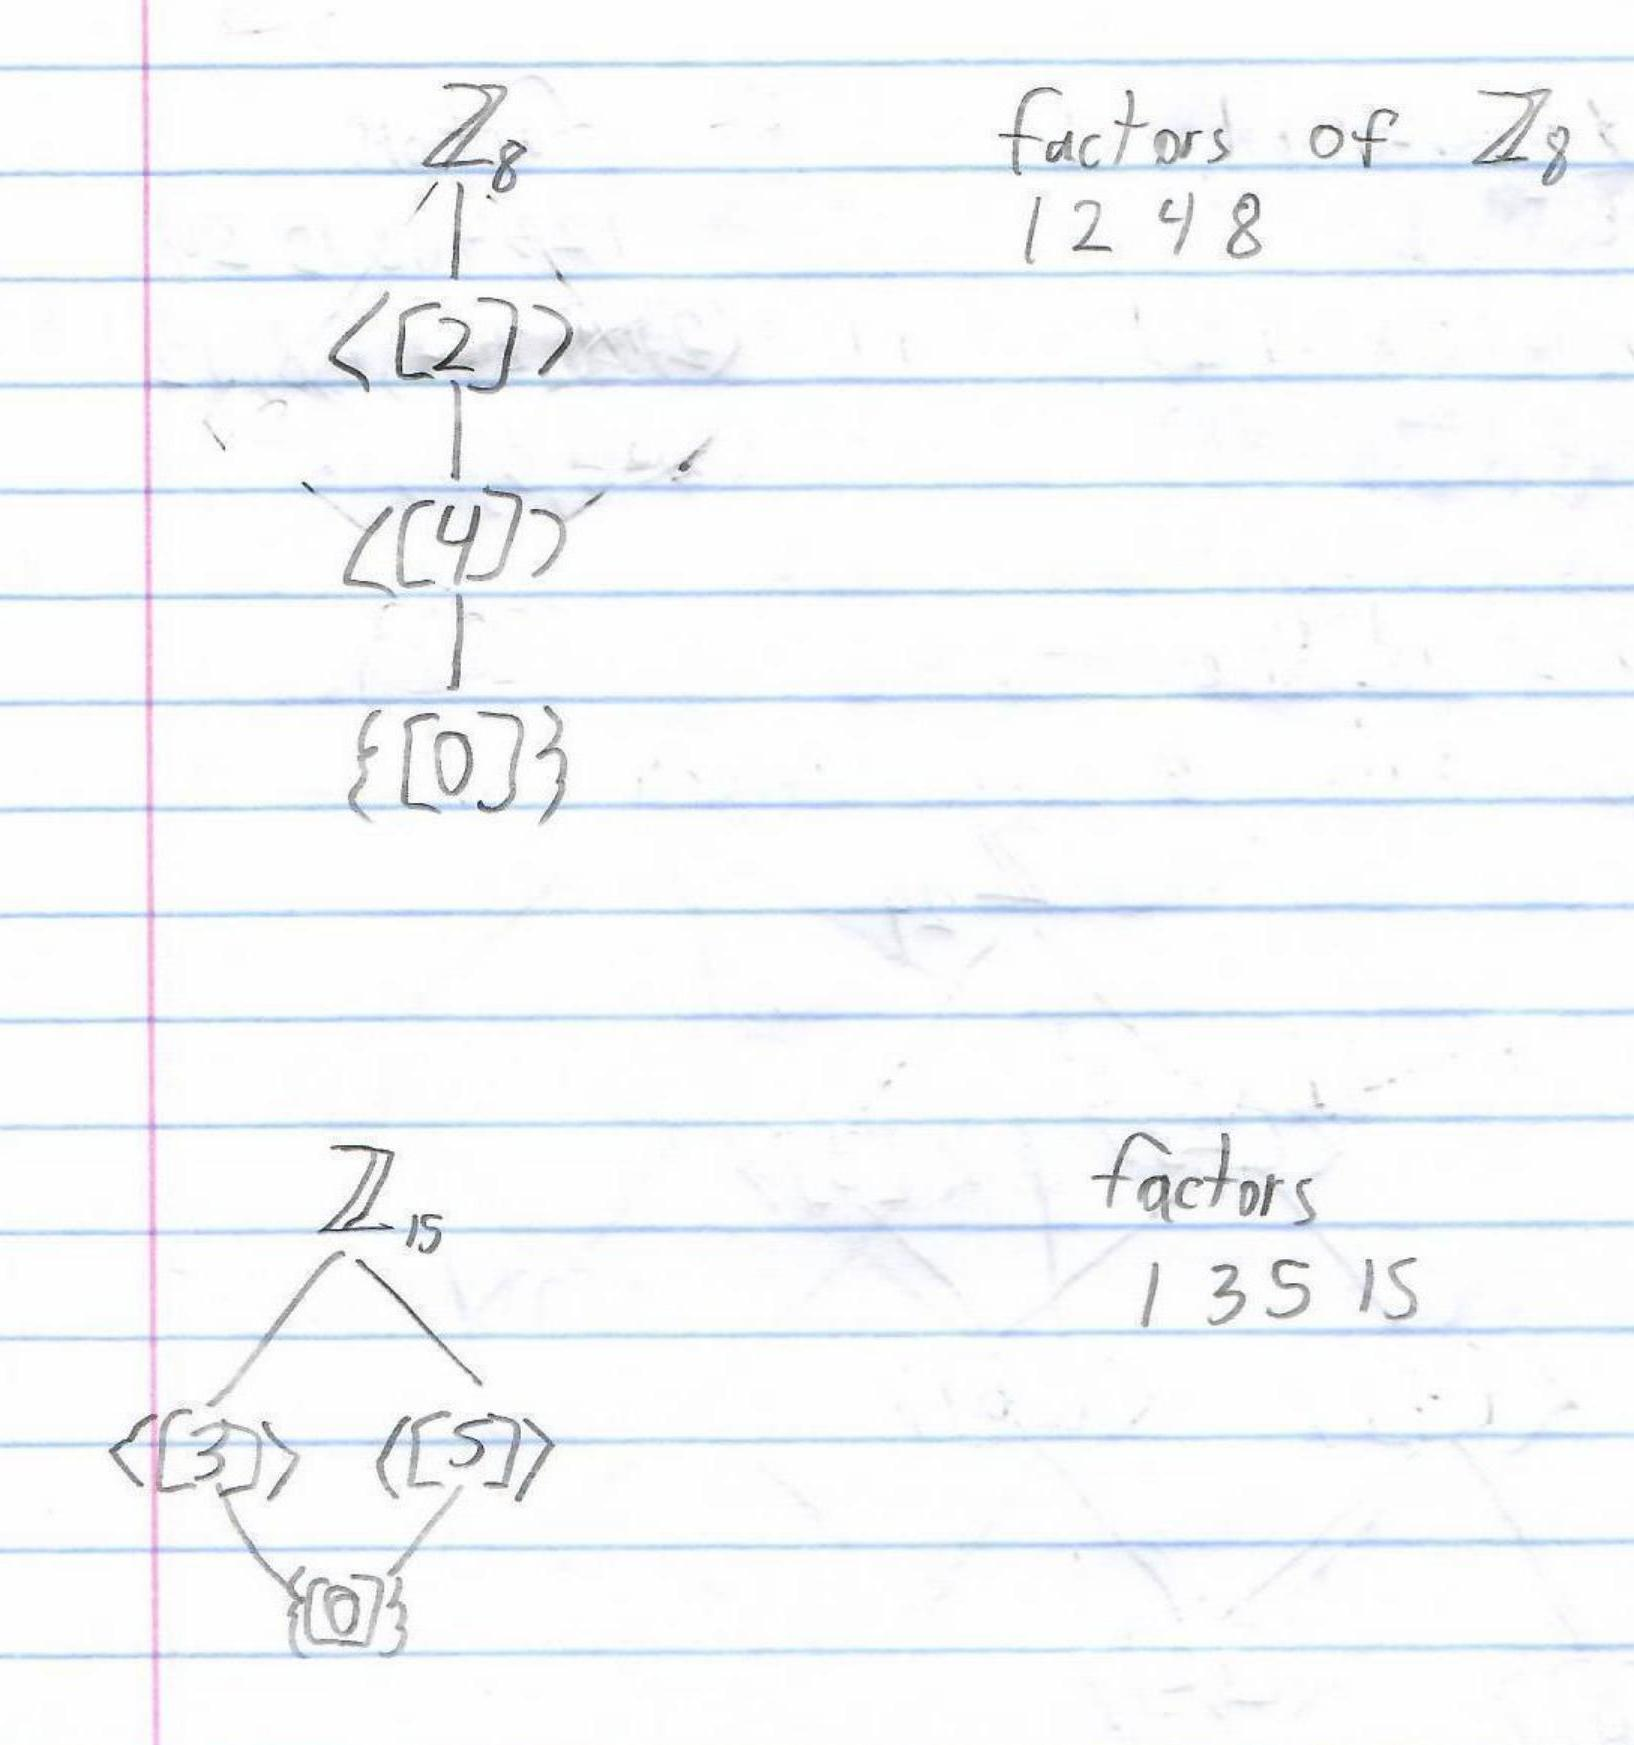
\includegraphics{lattice-Z8-Z15}
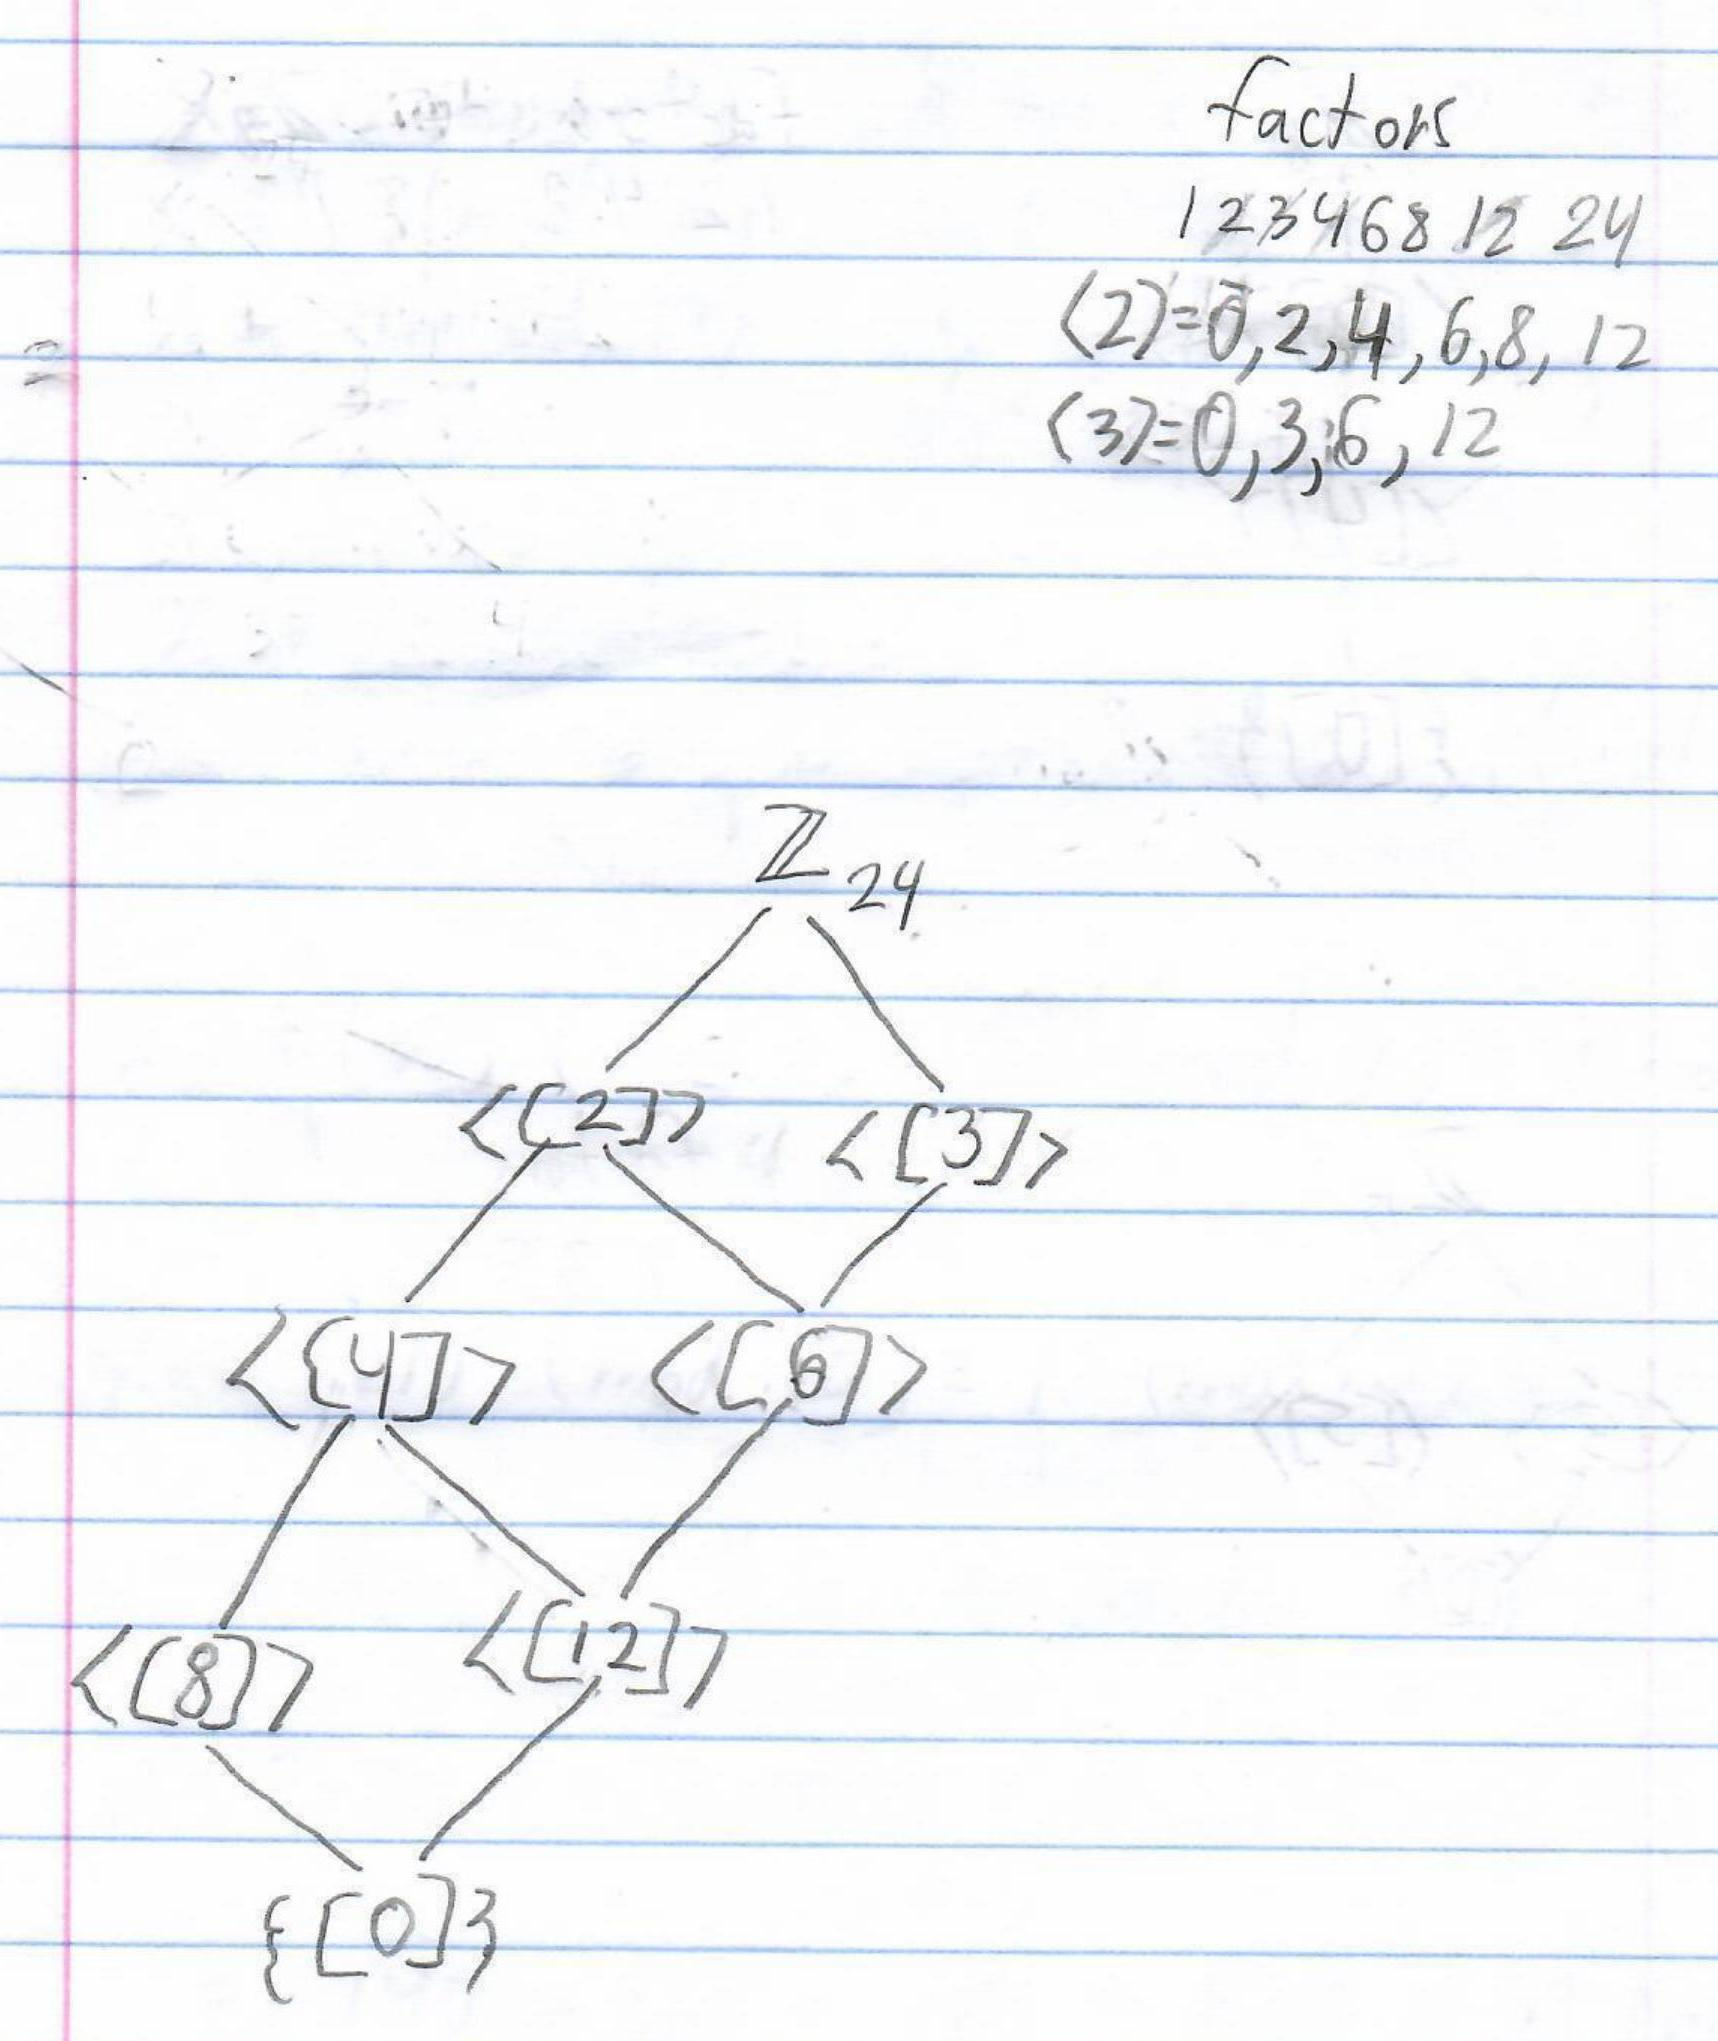
\includegraphics{lattice-Z24}
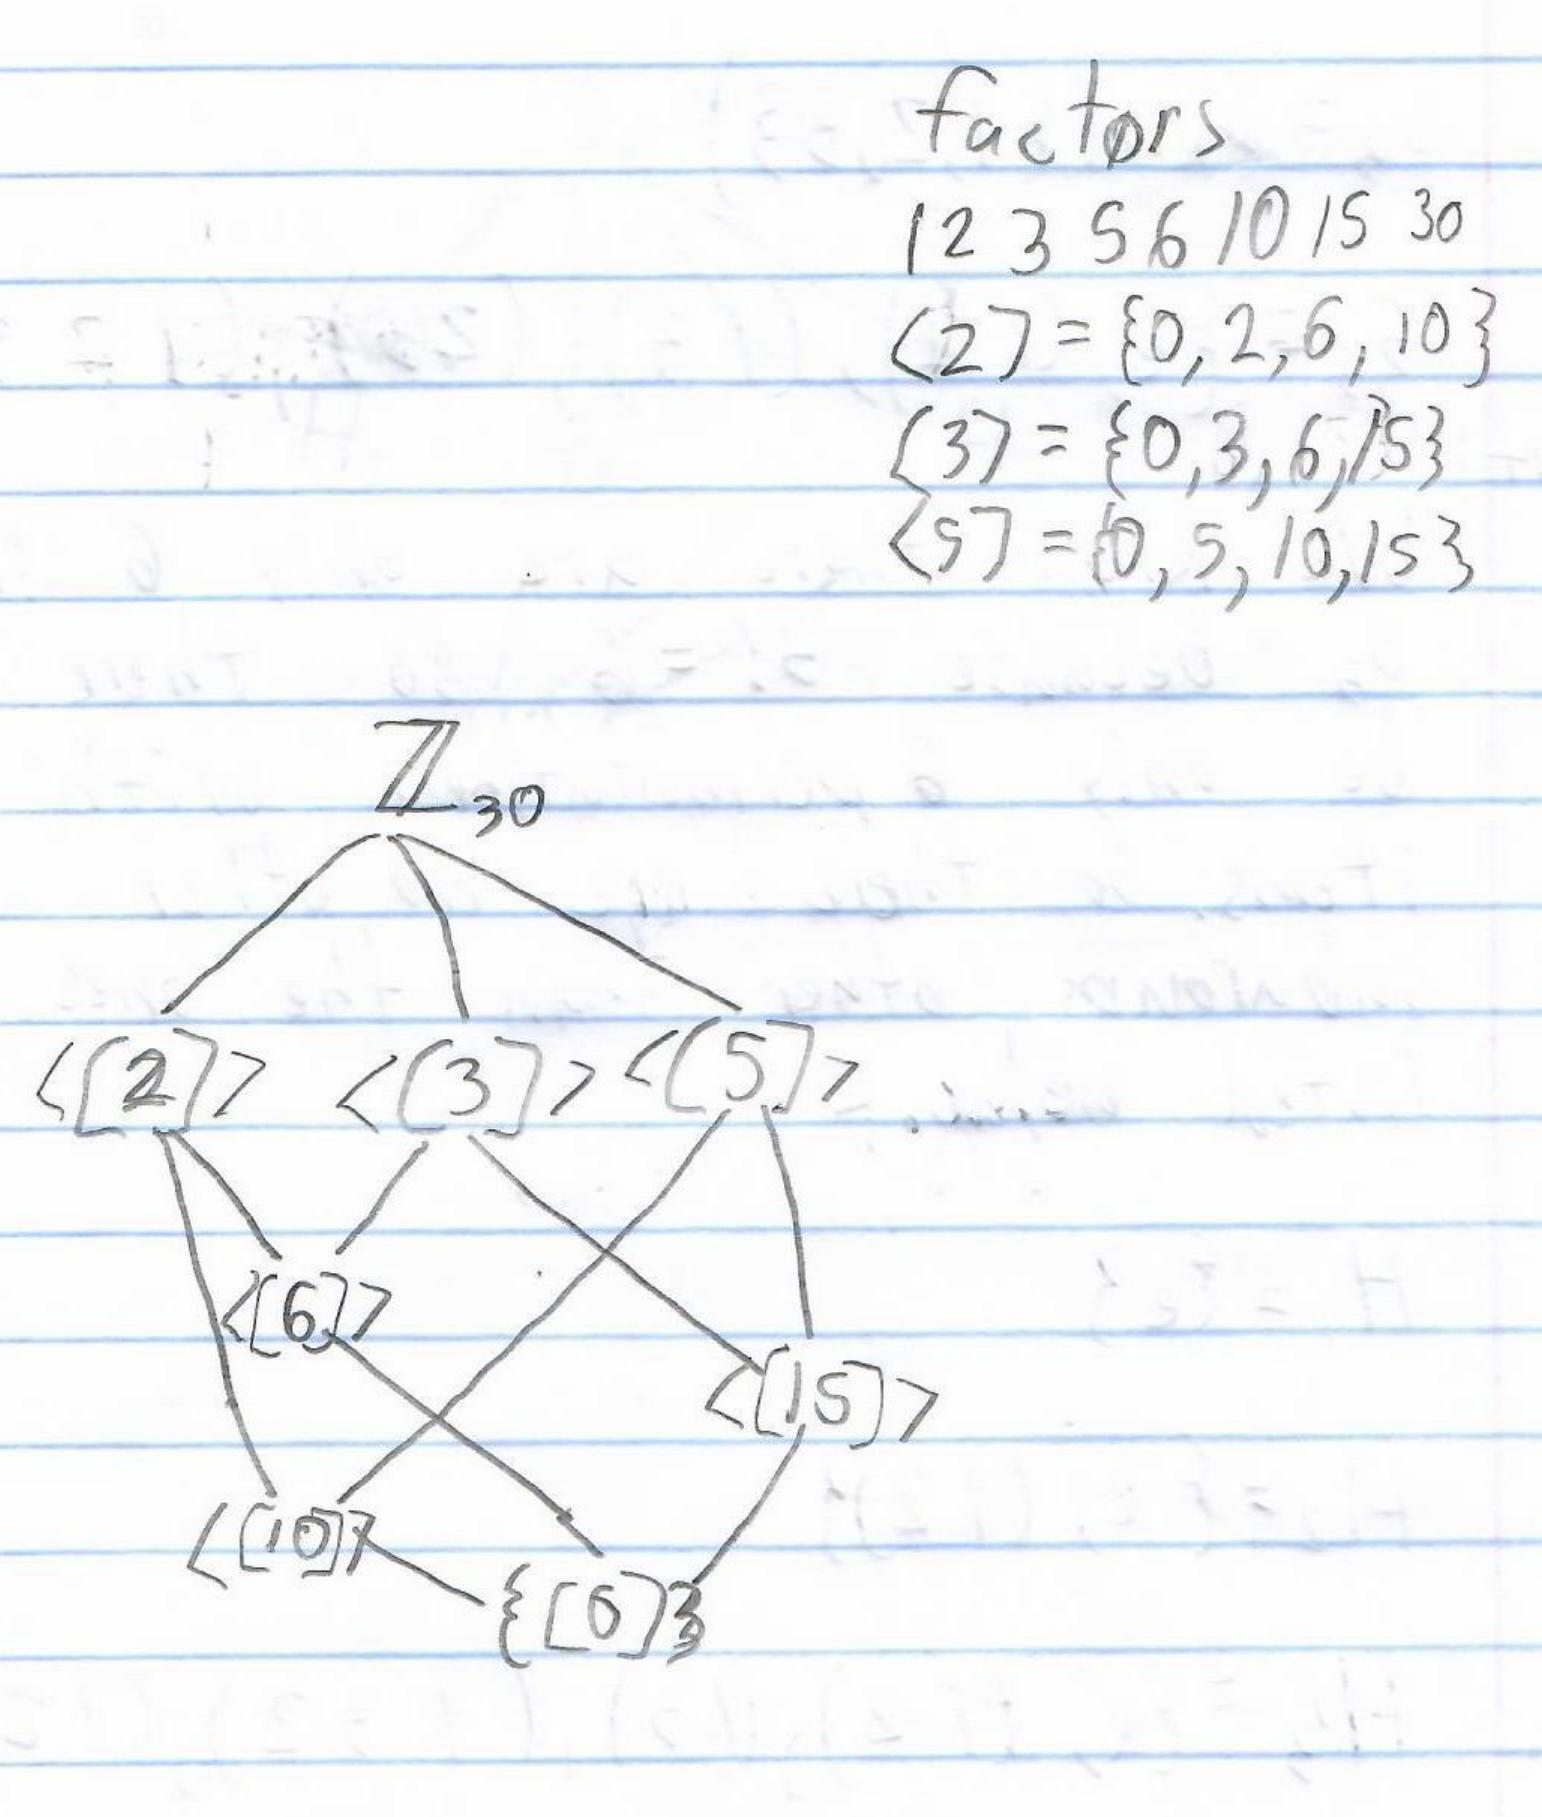
\includegraphics{lattice-Z30}

\textbf{Exercise 3.2.4}
Draw the subgroup lattice for $S_3$ (a group with respect to composition $\circ$).
You will need to find all the subgroups $H < S_3$ by hand (because we don't yet
have any theorems that tell us what the subgroups of $S_3$ are).
\textit{Hint: There are exactly 6 subgroups, but you should verify this by proving
that there are no other subgroups than the ones you have listed.}
\newline

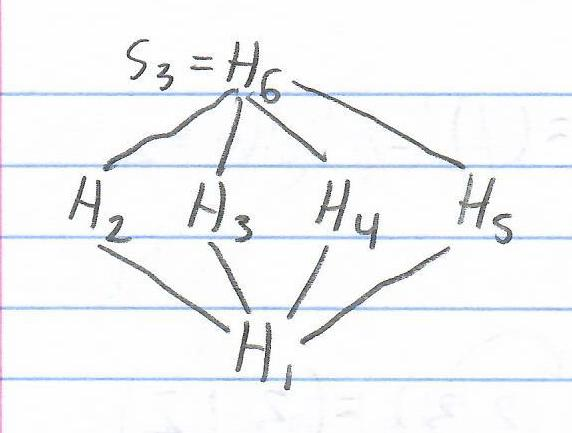
\includegraphics{lattice-S3}

\textbf{Exercise 3.2.5}
Prove that if $G$ and $H$ are groups and $K < G$, $J < H$ are subgroups, then
$K \times J \subset G \times H$ is a subgroup. Construct an example of a
subgroup of $\mathbb{Z}_2 \times \mathbb{Z}_2$ which is \textbf{not} of the form
$K \times J$ for some $K < \mathbb{Z}_2$ and $j < \mathbb{Z}_2$.

\end{myparindent}
\end{document}
